\documentclass[12pt]{article}
\usepackage{graphicx}
\begin{document}
	
\author{Houssem El Fekih}
\title{Big Data Processing - Coursework 1}
\maketitle

\section{Question 1}
In the map reduce job the mapper computes the real length of the tweet and then emits a record with key being the histogram bin (an IntWritable) corresponding to the length of a particular tweet and the value of 1. \\
The real Unicode character length is the count of Unicode code points.
The Java String object \emph{codePointCount(3)} Method returns the real length.
Then the correct histogram bin is computed by performing an euclidean division on that length by 5. \\
In the code there is also some logic that ensures the line being processed has 4 fields like it was specified in the question, to discard any bad data. \\
The raw results, obtained with getmerge from 2 reducers is in table. \ref{table:raw_results} \\
The requested histogram is shown in \ref{fig:length_tweets}

\begin{table}[h]
\centering
\caption{Unsorted frequency data}
\label{table:raw_results}
\begin{tabular}{ l r }
\hline
Histogram bin (1 -> 1-5 characters etc..) & Frequency \\
\hline
	2 &		10936 \\
	4 &		102779 \\
	6 &		320773 \\
	8 &		396311 \\
	10 &	482040 \\
	12 &	610254 \\
	14 &	715009 \\
	16 &	783543 \\
	18 &	906811 \\
	20 &	858255 \\
	22 &	974740 \\
	24 &	1086913 \\
	26 &	1409812 \\
	1 &		11964 \\
	3 &		33710 \\
	5 &		232401 \\
	7 &		356090 \\
	9 &		451583 \\
	11 &	527301 \\
	13 &	598994 \\
	15 &	690083 \\
	17 &	837353 \\
	19 &	936202 \\
	21 &	945548 \\
	23 &	1043816 \\
	25 &	1202640 \\
	27 &	9042688 \\
\end{tabular}
\end{table}

\begin{figure}
	\centering
	\caption{length of tweets histogram}
	\label{fig:length_tweets}
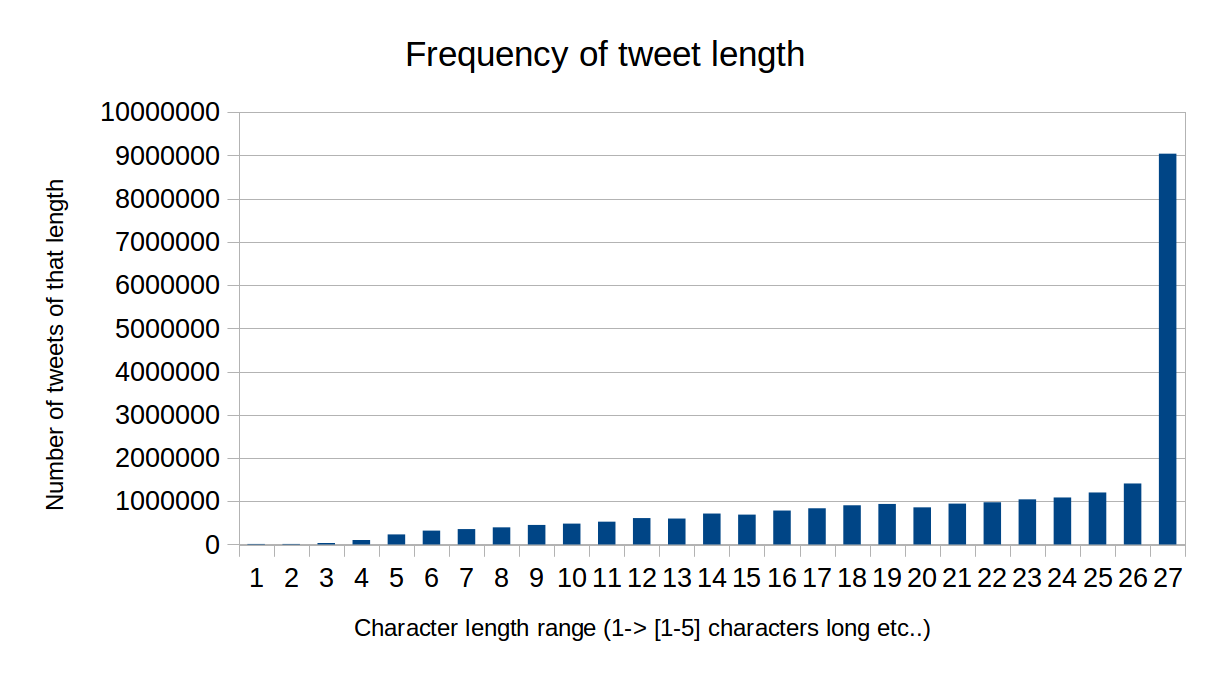
\includegraphics[width=10cm]{tweet_length_histogram.png}
\end{figure}

\section{Question 2 - part 1 - Tweets in hour}

As in all the questions, code is organised in packages, the package Q2P1
contains the code for part 1 of this question making class \emph{Q2P1.CW1TweetsInHourMapper} the main class for this question. \\

The first task in the mapper malformed lines are first discarded not containing the epoch after noticing some errors due to that. \\ 
There was no choice but to add a try catch block around parsing the time to avoid the map jobs failing which unfortunately is a performance penalty. \\
In order to retrieve the correct time JAVA 8 \emph{ZonedDateTime} and \emph{Instant} class are used with the timezone if of \emph{Brazil/East} which is where Rio is on. \\
The key emitted is the \emph{IntWritable(parsed hour)} and value is \emph{IntWritable(1)}.\\
The reducer is a summing reducer to add up all the instances of hours. \\ A combiner can be used in this case.
As it is shown on \ref{fig:tweets_time} the busiest hour is 23h00 which makes sense considering that the opening ceremony happen at that time and this event is the most hyped. \\
One other thing that one can notice is that although 11pm is 
higher in number of tweets by a big margin, all the data is in the same range of  1060000, this is because that this is a volume with a high number of watchers at any point but this uniformity might also be an artefact of the manner in which the data was collected. \\

\begin{figure}
	\centering
	\caption{tweets hour slot distribution histogram}
	\label{fig:tweets_time}
	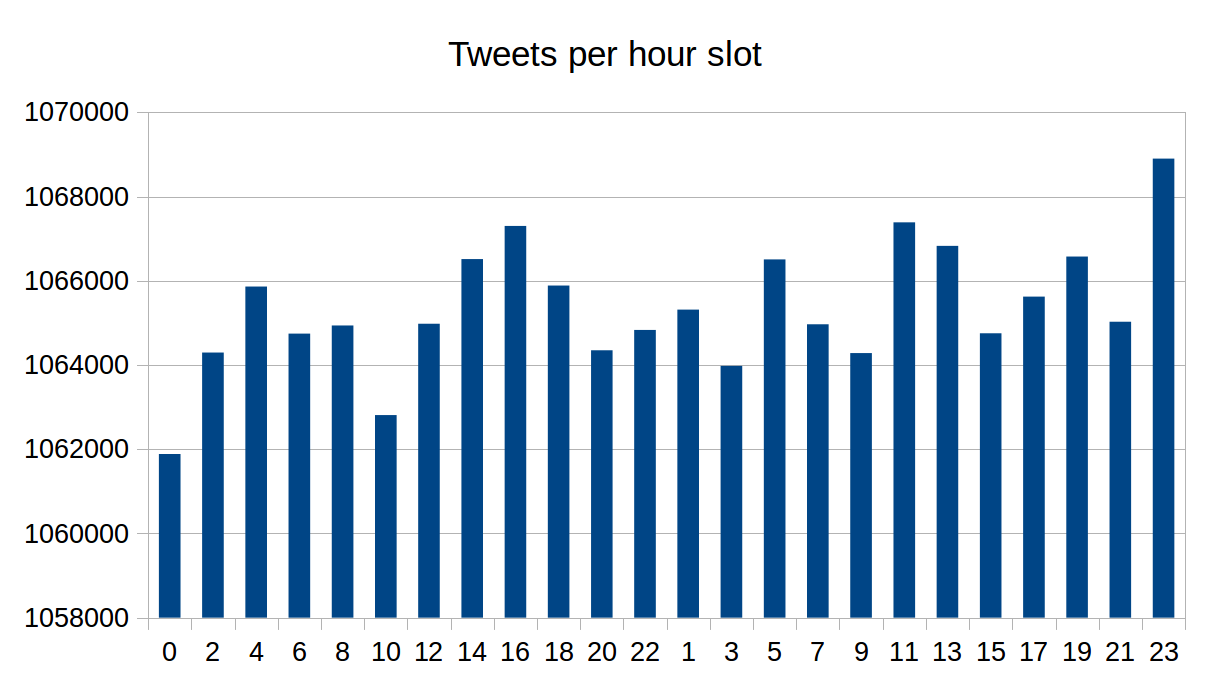
\includegraphics[width=10cm]{tweets_hour_slot}
\end{figure}

\section{Question 2 - part 2 Most popular hashtag in Busiest Hour}

As it was shown previous section the busiest time was 23h00. \\
The mapper first validates that the entry is a valid record, then
further filter any tweet that is not in the correct time slot. \\
It then emits as key all the matched hashtags with a count of one to the reducer . \\
The Mapper output type is (Text, IntWritable), the reducer aggregates those values.
It was difficult to choose an appropriate regexp for this exercise, one attempt was to
use a regexp excluding all non space characters like so: \\
\#[ (not \^)  \textbackslash s]+. \\
The problem with this approach is that JAVA's regexp handling does not understand all spaces in the unicode code page. \\
This lead to a lot of hashtags with Chinese or Russian containing spaces and text of the tweet. \\ There is also the added problem of punctuation, eg: "\#rio!" or more commonly "\#hashtag," \\
A simpler approach was opted for, which penalises all non-ascii hashtags in our analysis, which is a shame: "\#[\textbackslash w]+" \\
All of the sorting and histogram plotting was done with the help of libreoffice. \\

\begin{table}[ht]
\centering
\caption{Top 10 HashTags}
\label{table:top_hashtags}
\begin{tabular}{ l r }
\hline
HashTag & Count \\
\hline
\#Rio2016 &	842941 \\
\#rio2016 &	54232 \\
\#Olympics &	50442 \\
\#BRA &	21980 \\
\#USA &	20208 \\
\#Gold &	17963 \\
\#TeamUSA &	13845 \\
\#JuegosOlimpicos &	13791 \\
\#Futebol &	13402 \\
\#OpeningCeremony &	12786 \\
\end{tabular}
\end{table}

\section{Question 3 - Part 1}

This job sets up an ArrayList with the content being the full name of the athletes loaded from a cache file. \\
When parsing tweets we later iterate through all the elements of the list to try and find matches, for each match we emit as key the name of the artist and a count of one. \\
The reducer is another summing reducer and we can use a combiner for this task. Aggregation and filtering is done in LibreOffice. \\ 
The result is shown in table \ref{table:top_athletes}

\begin{table}[ht]
\centering
\caption{Top 30 Mentioned athletes}
\label{table:top_athletes}
\begin{tabular}{ l r }
\hline
Athlete & Count \\
\hline
neymar &	74693 \\
william &	12090 \\
luan &	5844 \\
michael phelps &	5190 \\
marquinhos &	1799 \\
simone biles &	1226 \\
usain bolt &	1206 \\
zeca &	435 \\
rafaela silva &	356 \\
ryan lochte &	351 \\
sakshi malik &	271 \\
ni yan &	261 \\
dan li &	230 \\
katie ledecky &	200 \\
teddy riner &	182 \\
weverton &	172 \\
li du &	155 \\
mariana pajon &	140 \\
ivan zaytsev &	138 \\
long ma &	125 \\
uilson &	104 \\
max whitlock &	93 \\
yulimar rojas &	84 \\
monica puig &	74 \\
azizulhasni awang &	73 \\
andy murray &	72 \\
gabriel jesus &	71 \\
liliyana natsir &	70 \\
adam peaty &	63 \\
ying han &	58 \\

\end{tabular}
\end{table}

\section{Question 3 - Part 2}
 
What this task requires us to do is to use the csv table to associate every mention with the sport associated with it. That is every time a mention is encountered, If it is relating to a particular athlete, the loaded data is looked up (this time it needs to be a HashMap of person to Sport) and a record is emitted with String(sport) and IntWritable(1). \\

Although an IntIntPair writer class is provided which would be useful to encode a value as well as a boolean value for determining if that entry is a key in reduce side join, A repartition join is unnecessary since the medalists data is small (a few 100kb in Hadoop scale) a map only join is adequate. \\

The reducer is a simple aggregating sum reducer. Sorting and taking top 10 The result is shown in table \ref{table:top_sports}\\
\begin{table}[ht]
\centering
\caption{Top 20 Mentioned sports}
\label{table:top_sports}
\begin{tabular}{ l r }
\hline
Sport & mentions of athletes in that sport \\
\hline
football &	9423 \\
aquatics &	645 \\
gymnastics &	178 \\
athletics &	174 \\
judo &	55 \\
volleyball &	47 \\
cycling &	44 \\
wrestling &	37 \\
tennis &	36 \\
table tennis &	32 \\
basketball &	18 \\
shooting &	14 \\
badminton &	14 \\
boxing &	11 \\
weightlifting &	8 \\
handball &	6 \\
fencing &	5 \\
equestrian &	4 \\
golf &	4 \\
hockey &	3 \\
\end{tabular}
\end{table}

\end{document}
